% !TEX program = xelatex

% 定义一个条件判断变量:打印模式
\newif\ifprint

% 设置是否打印,如果打印则执行 “插页” ,否则执行 “按顺序打印”
% 如果你不希望打印或是需要生成最后的校园图书馆(知网)发布版,可以取消注释这一行
\printtrue


\documentclass[a4paper,scheme=chinese,linespread=1.5]{ctexbook} % 行距固定值20磅
\usepackage[a4paper, top=2.54cm, bottom=2.54cm, left=3.18cm, right=3.18cm]{geometry} % 页边距 左右3.18cm 上下2.54cm
\setlength{\parskip}{0pt}  % 手动控制段落间距 

\usepackage{ctex}
\usepackage{arydshln} 

\usepackage{amsmath}
\usepackage{amssymb}

%\usepackage{newtxtext, newtxmath}

\usepackage{xeCJK}
\usepackage{xeCJKfntef}

\usepackage{fancyhdr}

\usepackage{tikz}
\usepackage{graphicx}

\usepackage{enumitem}
\usepackage{ragged2e}

% 五线谱包,可以用西贝柳斯+pdf代替
%\usepackage{musixtex}

\usepackage{float}

% 色彩库
\usepackage{xcolor}

% 设置页脚
\pagestyle{fancy}
\fancyhf{}  % 清空页眉和页脚
\renewcommand{\headrulewidth}{0pt} % 去除页眉横线
\renewcommand{\footrulewidth}{0pt} % 如果页脚横线也不需要,可以设置为 0pt

% 导入加载图片库
\usepackage{graphicx}
\usepackage{multicol}

\newcommand{\fixeduline}[2][8cm]{\uline{\makebox[#1]{#2}}}

\newcommand{\degree}{硕}%博 / 硕
\newcommand{\chimaintitle}{中文标题}
\newcommand{\chisubtitle}{——中文副标题} % 中文副标题 如果不用就去了 -> \newcommand{\chisubtitle}{}
\newcommand{\engtitle}{English Title}

% 导入时间
\usepackage{datetime2}

\usepackage{xparse}

% 表格
\usepackage{longtable}
\usepackage{multirow}
\usepackage{booktabs}

% 导入中文文献引用标准 GB/T 7714
\usepackage{gbt7714}
\bibliographystyle{gbt7714-numerical}

% 画表格或者画其他东西用
\usepackage{tikz}

%tikz库画圈
\newcommand*\circled[1]{\tikz[baseline=(char.base)]{
		\node[shape=circle,draw,inner sep=1.2pt] (char) {#1};}
} 

% 加载中文字体库
\usepackage{zhnumber}

% 阿拉伯对应中文数字的转换
%\newcommand{\chinesenumber}[1]{%
%	\ifcase#1 零 \or 一\or 二\or 三\or 四\or 五\or 六\or 七\or 八\or 九\or 十\fi
%}

\newcommand{\chinesenumber}[1]{%
	\zhnumber{\number#1}
}

\newcommand{\setenumChiNum}{%
	\setlist[enumerate,1]{%
		itemindent=2.6em,
		labelsep=0.25em,
		left=1.8em,
		itemsep=0.1em,
	}
}

\newcommand{\itemChiNum}{%
	\addtocounter{enumi}{1}
	\item [\text{(\zhnumber{\arabic{enumi}}})]
}

% 重置章节序号
\newcommand{\resetchapternum}{
	%\stepcounter{chapter}
	\setcounter{section}{0}
	\setcounter{subsection}{0}
	\setcounter{subsubsection}{0}
	\phantomsection
}

%\usepackage{ctex}
%\ctexset{chapter/name={第,章}, chapter/font=\Large\bfseries}

\NewDocumentCommand{\addabstract}{s m}{%
	\IfBooleanTF{#1}
	{
		%\addabstract*
		{		
			\begin{center}
				\zihao{-2} \bfseries #2
			\end{center}
			\addcontentsline{toc}{chapter}{英文摘要}
			
		}
	} % * 英文标题样式
	{
		%\addabstract
		\stepcounter{chapter}
		{
			\begin{center}
				\zihao{-2} \heiti #2
			\end{center} 
			\addcontentsline{toc}{chapter}{中文摘要}
			
		}
	} % 中文标题样式
	
	% 设置chapter序号从0开始
	\setcounter{chapter}{0}
}

\NewDocumentCommand{\addchapter}{s m}{%
	\IfBooleanTF{#1}
	{
		%\addchapter*
		{
			\begin{center}
				\zihao{-2} \heiti  #2
			\end{center}
		}
		\addcontentsline{toc}{chapter}{#2}
	} % * 不增加章
	{
		%\addchapter
		\stepcounter{chapter}
		{
			\begin{center}
				\zihao{-2} \songti 第\chinesenumber{\value{chapter}}章、#2
			\end{center}
		}
		\addcontentsline{toc}{chapter}{第\chinesenumber{\value{chapter}}章\quad #2}
	} % 增加章
	\resetchapternum
}

% 页面设置
\usepackage{titlesec}
\usepackage{tocloft}
%\usepackage{fontspec}
%\usepackage[subfigure]{tocloft}

% 自定义 目录
\setcounter{tocdepth}{4}
\renewcommand{\contentsname}{\vspace*{-2.35em} \hfill \zihao{-2}\color{black}目~~~录 \hfill}  % 修改目录的标题 居中 小二 黑体

\renewcommand{\cftchapleader}{\cftdotfill{\cftdotsep}} % 目录加省略号

\setlength{\cftsecindent}{3em}  % 设置 section 的缩进为 3.5em
\setlength{\cftsubsecindent}{5em}  % 设置 subsection 的缩进
\setlength{\cftsubsubsecindent}{7.5em}  % 设置 subsection 的缩进

\setlength{\cftsecnumwidth}{4em}  % 设置章节编号宽度
\setlength{\cftsubsecnumwidth}{4em}  % 设置子章节编号宽度
\setlength{\cftsubsubsecnumwidth}{4em}  % 设置子章节编号宽

% 分页
\usepackage{afterpage}

% 打印时增加页数
\usepackage{xstring}

% 页码差计数器
\newcounter{CalcPageDiff}

% 大写罗马页码数字计数器
\newcounter{Romancounter}
\newcommand{\RomannumToArabic}[1]{
	\setcounter{Romancounter}{0}% 计数器置零
	\foreach \i in {1, 2, 3, 4, 5, 6, 7, 8, 9, 10} {%
		\IfStrEqCase{#1}{%
			{\uppercase\expandafter{\romannumeral\i}}{\setcounter{Romancounter}{\i}}% 大写罗马字符 I II III IV V VI VII VIII IX X
			{\romannumeral\i}{\setcounter{Romancounter}{\i}}% 小写罗马字符 i ii iii iv v vi vii viii ix x 
		}[\PackageWarning{Romconvert}{Invalid input: #1}]% 非法输入
	}
	%\arabic{Romancounter}%
}

% 超链接
\usepackage{hyperref}
\hypersetup{
	pdfborder={0 0 0},        % 边框为无(无边框)
	colorlinks=false,          % 启用彩色链接
	linkcolor=white,           % 章节、表格、图形的链接颜色
	citecolor=white,           % 引用的链接颜色
	urlcolor=white,            % URL 的链接颜色
	pdfauthor={},             % 作者
	pdftitle={},              % 标题
	pdfsubject={},            % 主题
	pdfkeywords={},           % 关键词
	pdfcreator={},            % 创建者
	pdfproducer={},           % 生产者
	%linkbordercolor=black,      % 设置链接的边框颜色
	%urlbordercolor=black,           % 设置URL的边框颜色
	%citebordercolor=black,            % 设置引用的边框颜色
	%pdfborderstyle={/S/D/D[3 2]/W 1} % 虚线
}

% 脚注
\usepackage{pifont}  % 引入宏包pifont,用于设置带圈数字
\usepackage{footnote}
\usepackage[perpage]{footmisc}

% 需结合计数器调整:
\renewcommand{\thefootnote}{%
	\ifnum\value{footnote}<11 
	\raisebox{0.35ex}{\scalebox{0.75}{\ding{\numexpr 171+\value{footnote}}}}% 缩放符号 ①~⑩
	\else 
	\textcircled{\scriptsize\arabic{footnote}}% 超过11时改用其他方式
	\fi}

% 伪代码
%\usepackage{algorithm}
%\usepackage{algorithmic}
%\usepackage{algpseudocode}
\usepackage[linesnumbered,ruled,vlined]{algorithm2e}



% 自定义 section 标题:第x节
\renewcommand{\thesection}{第\chinesenumber{\value{section}}节}
\titleformat{\section}%[block]
{	
	\centering
	\raggedright
	\zihao{3}
}
{}{0em}{}
\newcommand{\DIYsection}[1]{
	\stepcounter{section}
	%
	\section*{
		\zihao{3}
		\begin{center}
			\thesection、
			#1
		\end{center}
		\vspace*{-2.5em}
	}
	
	\addcontentsline{toc}{section}{\thesection \quad #1}
}

% 自定义 subsection 标题: 一、二、三... [可自行修改]
\renewcommand{\thesubsection}{\chinesenumber{\value{subsection}}}
\titleformat{\subsection}%[block]
{	
	\raggedright
	\songti
	\zihao{-3}
	\color{black}
}
{}{0em}{}
\newcommand{\DIYsubsection}[1]{
	\stepcounter{subsection}
	\subsection*{\thesubsection、#1}
	\addcontentsline{toc}{subsection}{\thesubsection、#1}
}


% 图表注释
\usepackage{caption}
\captionsetup{labelfont={rm, bf,color=black},textfont={rm,bf}}

%图表脚注
\usepackage{tablefootnote}

%字体设置
\newCJKfontfamily\huawenzhongsong{STZHONGS}[BoldFont=STZHONGS, Path=./fonts/, Extension=.TTF] %华文中宋
\setmainfont{Times New Roman} % 设置西文字体 
\setCJKmainfont[
BoldFont = SimHei
]{SimSun}       % 设置中文字体为宋体 



\begin{document}

	% TODO 封面信息
	\begin{titlepage}
		\begin{center}
			\noindent
			
\includegraphics[width=0.6\textwidth]{figures/ccom/ccom_logo.eps}\vspace{2cm}
		\end{center}
		
		
		\begin{center}
			{\fontsize{36pt}{36pt}\fontfamily{微软雅黑}\selectfont \degree~\:士~\:学~\:位~\:论~\:文}\vspace{2cm}
			
			{ \heiti \fontsize{32pt}{32pt}\selectfont\bfseries \chimaintitle \protect\\
				\vspace*{0.25em}
				\fontsize{28pt}{28pt}\selectfont\bfseries \chisubtitle \par}%\vfill
			
			\vspace*{10em}
			{\LARGE\huawenzhongsong
				作者姓名:\fixeduline{匿名}\\
				学  号:\fixeduline{2XXXXX}\\
				所在系部:\fixeduline{音乐人工智能与音乐信息科技}\\
				研究方向:\fixeduline{音乐人工智能与音乐信息科技}\\
				导师姓名:\fixeduline{YF~教授、XXX~教授}\\
				提交时间:\fixeduline{20XX年04月}\\
			}
		\end{center}
		
	\end{titlepage}
	
	\ifprint
	% 如果是打印模式,判断是否需要加一页
		\newpage
		\null\
		\thispagestyle{empty} % 禁用页码
		\newpage
	\else
	% 如果不是打印模式,则不改变
	\fi
	
	% TODO 论文原创性声明和使用授权书
	{\large
		
		\setlength{\columnsep}{0pt}
		
		{
			\centering 
			\fontsize{16pt}{16pt}
			\heiti{中央音乐学院\degree 士学位论文原创性声明}\par
		}
		
		\vspace{0.3cm}
		
		本人郑重声明:此处所提交的\degree 士学位论文\kaishu \uline{\,《\chimaintitle\chisubtitle》} \songti ,是本人在导师指导下,在中央音乐学院攻读\degree 士学位期间独立进行研究工作所取得的成果。据本人所知,论文中除已注明部分外不包含他人已发表或撰写过的研究成果。对本文的研究工作做出重要贡献的个人和集体,均已在文中以明确方式注明并表示了谢意。本声明的法律结果将完全由本人承担。
		
		\begin{multicols}{2}
			\vfill\null
			\columnbreak
			\heiti{作者签名:}~~~~%\raisebox{-0.2\height}{\includegraphics[width=1.25cm, height=0.65cm ]{figures/signatures/sy.pdf}} % 括号里是作者电子签
			\par
			\vspace{0.3cm}
		\end{multicols}
		
		\hfill \heiti{\the\year~年~\the\month~月~\the\day~日}
		\vfill
		
		{
			\centering 
			\fontsize{16pt}{16pt}
			\heiti{中央音乐学院\degree 士学位论文使用授权书}\par
		}
		
		\vspace{0.3cm}
		
		\songti
		
		\kaishu \uline{\,《 {\chimaintitle\chisubtitle}》} \songti 系本人在中央音乐学院攻读\degree 士学位期间在导师指导下完成的\degree 士学位论文。本人完全了解中央音乐学院关于保存、使用学位论文的规定,同意学校保留并向有关部门送交论文的复印件和电子版本,允许论文被查阅和借阅。
		
		\begin{multicols}{2}
			\vfill\null
			%\columnbreak
			\heiti{作者签名:}~~~~%\raisebox{-0.25\height}{\includegraphics[width=1.25cm, height=0.65cm ]{figures/signatures/sy.pdf}} % 括号里是作者电子签
			
			\vspace*{0.3cm}
			\hfill \heiti{\the\year~年~\the\month~月~\the\day~日}
			\vfill
			
			\columnbreak
			
			\vfill\null
			
			\heiti{导师签名: }\raisebox{-0.35\height}{
\includegraphics[width=1.75cm, height=1cm ]{figures/signatures/yuyuan.pdf}} \quad %\raisebox{-0.25\height}{\includegraphics[width=1.75cm, height=1cm ]{figures/signatures/dls.pdf}} % 二位导师签名
			
			\vspace*{0.3cm}
			\hfill \heiti{\the\year~年~\the\month~月~\the\day~日}
			
			\vfill
		\end{multicols}
		
		\vfill
		
		{
			\centering 
			\fontsize{16pt}{16pt}
			\heiti{中央音乐学院\degree 士学位论文使用授权书}\par
		}
		
		\vspace{0.3cm}
		
		本人授权中央音乐学院,可以将本论文提交中国学术期刊(光盘版)电子杂志社在《中国优秀博硕士学位论文数据库》中发表,可以采用影印、缩印或扫描等复制手段保存学位论文。
		
		\begin{multicols}{2}
			\vfill\null
			%\columnbreak
			\heiti{作者签名:}~~~~%\raisebox{-0.25\height}{\includegraphics[width=1.25cm, height=0.65cm ]{figures/signatures/sy.pdf}} %括号里是作者电子签
			
			\vspace*{0.3cm}
			\hfill \heiti{\the\year~年~\the\month~月~\the\day~日}
			\vfill
			
			\columnbreak
			
			\vfill\null
			
			\heiti{导师签名: }\raisebox{-0.35\height}{
\includegraphics[width=1.75cm, height=1cm ]{figures/signatures/yuyuan.pdf}} \quad %\raisebox{-0.25\height}{\includegraphics[width=1.75cm, height=1cm ]{figures/signatures/dls.pdf}} %二位导师签名
			
			\vspace*{0.3cm}
			\hfill \heiti{\the\year~年~\the\month~月~\the\day~日}
			
			\vfill
		\end{multicols}
	
	}
	
	\ifprint
	% 如果是打印模式,判断是否需要加一
		\newpage
		\null\
		\thispagestyle{empty} % 禁用页码
		\newpage
	\else
	% 如果不是打印模式,则不改变
	\fi
	
	\newpage
	
	% 中文摘要
	% 正文前可设置页码为小写罗马数字 
	\pagenumbering{roman}
	\fancyfoot[C]{\thepage}
	\setcounter{page}{1}
	% 定义中文摘要开头
	\label{chinese_abstract_start}
	\addabstract{论文摘要}
	{
		这里写中文摘要。
		
		
		\bigskip
		\textbf{关键词}: % 中文关键词,用;隔开,3~6个为宜
		音乐;深度学习;神经网络
	}
	
	% 定义中文摘要结尾
	\label{chinese_abstract_end}
	\ifprint
	% 如果是打印模式,判断是否需要加一页
	\afterpage{% 延迟执行页码判断 页码差为奇数就增加一页空白页,偶数不动
		\RomannumToArabic{\getpagerefnumber{chinese_abstract_end}}
		\setcounter{CalcPageDiff}{\value{Romancounter}}
		\RomannumToArabic{\getpagerefnumber{chinese_abstract_start}}
		\addtocounter{CalcPageDiff}{-\value{Romancounter}}		
		
		\ifodd \arabic{CalcPageDiff}
			
		\else
			\newpage
			\null\
			\thispagestyle{empty} % 禁用页码
			\newpage
			\setcounter{page}{\value{page}-1}
		\fi
		
	}
	\else
	% 如果不是打印模式,则不改变
	\fi
	
	\newpage
	
	% 英文摘要
	% 定义英文摘要开头
	\newcommand{\EnglishAbstractStart}{\arabic{page}}
	\label{english_abstract_start}
	\addabstract*{\textbf{Abstract}}
	{
		Write an English abstract here.
		
		
		\bigskip
		\textbf{Key Words}: % 英文关键词,首字母大写,用;隔开
		Music; Deep Learning; Neural Network
	}
	
	% 定义英文摘要结尾
	\newcommand{\EnglishAbstractEnd}{\arabic{page}}
	\label{english_abstract_end}
	\ifprint
	% 如果是打印模式,判断是否需要加一页
	\afterpage{% 延迟执行页码判断 页码差为奇数就增加一页空白页,偶数不动
		\RomannumToArabic{\getpagerefnumber{english_abstract_end}}
		\setcounter{CalcPageDiff}{\value{Romancounter}}
		\RomannumToArabic{\getpagerefnumber{english_abstract_start}}
		\addtocounter{CalcPageDiff}{-\value{Romancounter}}		
		
		\ifodd \arabic{CalcPageDiff}
		
		\else
		\newpage
		\null\
		\thispagestyle{empty} % 禁用页码
		\newpage
		\setcounter{page}{\value{page}-1}
		\fi
		
	}
	\else
	% 如果不是打印模式,则不改变
	\fi
	
	\newpage
	
	% 生成目录
	\label{contents_start}
	\tableofcontents
	\label{contents_end}
	
	\ifprint
	% 如果是打印模式,判断是否需要加一页
		\afterpage{% 延迟执行页码判断 奇数就增加一页空白页,偶数不动
			\RomannumToArabic{\getpagerefnumber{contents_start}}
			\setcounter{CalcPageDiff}{\value{Romancounter}}
			\RomannumToArabic{\getpagerefnumber{contents_end}}
			\addtocounter{CalcPageDiff}{-\value{Romancounter}}		
			
			\ifodd \arabic{CalcPageDiff}
			\else
			\newpage
			\null\
			\thispagestyle{empty} % 禁用页码
			\newpage
			\setcounter{page}{\value{page}-1}
			\fi
			
		}
	\else
	% 如果不是打印模式,则不改变
	\fi
	
	\newpage
	
	% 恢复页码
	\fancyhf{}
	\pagenumbering{arabic}
	\fancyfoot[C]{\thepage}
	\setcounter{page}{1}
	
	% 绪论
	\addchapter*{绪\quad 论}
	请在此处写绪论。
	
	\DIYsection{研究背景与意义}
	应该研究什么问题呢?
	
	\newpage
	
	\addchapter{这是“第一章”:一级标题chapter}
	
	\DIYsection{这是“第一节”:二级标题section}
	
	\DIYsubsection{这是“一、”:三级标题subsection}
	
	\setenumChiNum
	\begin{enumerate}
		\itemChiNum 
		这是“(一)”:四级标题,使用enumerate驱动。
		
	\end{enumerate}
	
	脚注这样标\footnote{李伟、王鑫主编:《音频音乐与计算机的交融——音频音乐技术2》,上海:复旦大学出版社,2022年,第252-270页。}。
	
	% 这是图片
	\begin{figure}[H]
		\centering
		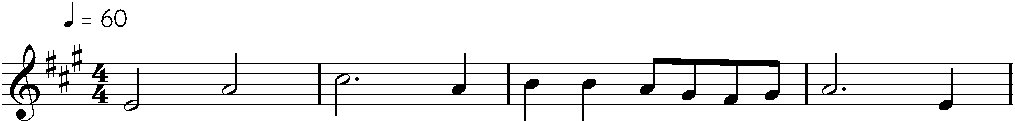
\includegraphics[width=1\textwidth]{figures/vio1_beeth2_1.pdf}  % 插入PDF文件
		\caption{图片标题}  % 图片标题
		\label{fig:1.1}  % 图片标签
	\end{figure}
	
	使用“\textbf{$\backslash \text{ref\{fig:1.x\}}$}”引用公式\ref{fig:1.1}。使用“$\backslash \text{toprule}[\text{1.5pt}]$”和“$\backslash \text{bottomrule}[\text{1.5pt}]$”来定义表格顶部和底部的线宽,使用“$\backslash \text{midrule}[\text{0.75pt}]$”定义中间线宽,以此基准制作三线格。可使用“$\backslash \text{cmidrule}[{line\ width}]\{{number}_1-{number}_2\}$”自定义线宽和占据的格数,如表\ref{tab:1.2}第三行所示。
	
	表格生成可通过\href{https://www.tablesgenerator.com/}{\tikz[baseline=-0.375em] \node[rounded corners=5pt, fill=yellow!25, text=black]{\textbf{\LaTeX 在线表格生成器}\textit{(点击链接跳转)}};}进行生成。
	
	% 这是表格
	\begin{table}[h]
		\centering
		\caption{表格标题}
		\vspace*{-1em}
		\begin{tabular}{ccccccc}
			\toprule[1.5pt]
			Pitch (MIDI) & Onset & Duration  & String & Position & Finger & Type \\ \midrule[0.75pt]
			64           & 0     & 2         & 2 	  & 1 		 & 2 	  & 1 \\
			69           & 2     & 2         & 2 	  & 3		 & 3 	  & 1 \\
			73           & 0     & 3         & 2 	  & 3 		 & 5 	  & 1 \\
			69           & 3     & 1         & 2 	  & 3 		 & 3 	  & 1 \\
			71           & 0     & 1         & 2 	  & 3 		 & 4 	  & 1 \\
			71           & 1     & 1         & 2 	  & 3 		 & 4 	  & 1 \\
			69           & 2     & 0.5       & 2 	  & 3 		 & 3 	  & 1 \\
			68           & 2.5   & 0.5       & 2 	  & 2 		 & 3 	  & 1 \\
			66           & 3     & 0.5       & 2 	  & 2 		 & 2 	  & 1 \\
			68           & 3.5   & 0.5       & 2 	  & 2 		 & 3 	  & 1 \\
			69           & 0     & 3         & 2 	  & 2 		 & 4 	  & 1 \\
			64           & 3     & 1         & 2 	  & 1 		 & 2 	  & 1 \\ 
			\bottomrule[1.5pt]
		\end{tabular}
		\label{tab:1.1}
	\end{table}
	
	\newpage
	
	展示一下公式的写法。可通过\href{https://www.latexlive.com/}{\tikz[baseline=-0.375em] \node[rounded corners=5pt, fill=pink!35, text=black]{\textbf{\LaTeX 在线公式编辑器}\textit{(点击链接跳转)}};}进行编写。
	
	% 这是公式
	\begin{align}
		M_{noise\_new}(f,t)= \frac{1}{2k+1} \sum_{t'=t-k}^{t+k} M_{noisy}(f,t')
		\label{equ:1.1}
	\end{align}
	
	\begin{equation}
		P_{enhanced}(f,t)= \left( P_{noise\_new}(f,t)^\gamma - \alpha P_{noise}(f)^\gamma \right)^{1/\gamma}
		\label{equ:1.2}
	\end{equation}
	
	使用“\textbf{$\backslash \text{ref\{equ:1.x\}}$}"引用单号公式\ref{equ:1.1}、多行公式\ref{equ:1.2}。
	
	\newpage
	
	如表\ref{tab:1.2}所示,展示一下表格内脚注的使用方法:“$\backslash \text{footnotemark}\{\}$”和“$\backslash \text{footnotetext\{\}}$”以及“$\backslash \text{addtocounter} \backslash \text{\{footnote\}\{1\}}$”,假设已经提到了DWPose\footnote{Zhendong Yang, Ailing Zeng, Chun Yuan, et al., \textit{``Effective Whole-body Pose Estimation with Two-stages Distillation''}, \textit{Proceedings of the 2023 IEEE/CVF International Conference on Computer Vision Workshops}, 2023, pp. 4212-4222.}。$\backslash \text{footnotemark} [ 1 ]\{\}$中的方括号[]如果带有数字(如[1]),则搭配$\backslash \text{setcounter\{footnote\}\{}\mathnormal{num}\text{\}}$使用时,脚注上标从$num$开始;反之,不使用[]时,则从$num+1$开始。
	
	PyTorch\footnote{PyTorch官网用户手册:\href{https://pytorch.org/docs/stable/index.html}{https://pytorch.org/docs/stable/index.html}}是一个用于机器学习和深度学习的开源深度学习框架,由Meta(Facebook)于2016年发布。以此为例展示混编脚注和脚注超链接功能(使用$\backslash \text{href\{URL\}\{text\}}$表示),将鼠标移到下方脚注\footnotemark[2]{}或者移动到后面的链接位置,都可以点击链接弹出浏览器转到相关页面。链接:\href{https://pytorch.org/docs/stable/index.html}{https://pytorch.org/docs/stable/index.html}
	
	
	\begin{table}[H]
		\centering
		\caption{人体姿态估计模型性能对比}
		\vspace*{-1em}
		\begin{tabular}{ccccc} %{|c|c|c|c|c|c|c|}%
			\toprule[1.5pt]
			模型   &  平均精度(AP) & 手部检测优化 & 实时性 & 模型大小 \\ \midrule[0.75pt]
			\setcounter{footnote}{1}
			DWPose\footnotemark[2]{}    & 0.665      & \checkmark                 & 中高       & 轻量级         \\
			\setcounter{footnote}{3}
			RTMPose\footnotemark[1]{}     & 0.653      & $\times$                & 高      &  中等          \\
			OpenPose\footnotemark{}    & 0.600        & $\times$                & 底       &  较大            \\ \cmidrule[0.5pt]{1-2}
			MediaPipe\footnotemark{}     & /      &  \checkmark                 & 极高       &  极小        \\
			\bottomrule[1.5pt]
		\end{tabular}
		\label{tab:1.2}
	\end{table}
	
	% DWPose
	%\setcounter{footnote}{2}
	%\footnotetext{Zhendong Yang, Ailing Zeng, Chun Yuan, et al., \textit{``Effective Whole-body Pose Estimation with Two-stages Distillation''}, \textit{Proceedings of the 2023 IEEE/CVF International Conference on Computer Vision Workshops}, 2023, pp. 4212-4222.}
	
	% RTMPose
	\setcounter{footnote}{3}
	\footnotetext{Tao Jiang, Peng Lu, Li Zhang, et al., \textit{``RTMPose: Real-Time Multi-Person Pose Estimation based on MMPose''}, \textit{arXiv:2303.07399}, 2023, pp. 1-11.}
	
	% OpenPose
	\addtocounter{footnote}{1}
	\footnotetext{Zhe Cao, Gines Hidalgo, Tomas Simon, et al., \textit{``OpenPose: Realtime Multi-Person 2D Pose Estimation using Part Affinity Fields''}, \textit{IEEE Transactions on Pattern Analysis and Machine Intelligence}, 2019, 43(1). pp. 172-186.}
	
	% Mediapipe
	\addtocounter{footnote}{1}
	\footnotetext{Camillo Lugaresi, Jiuqiang Tang, Hadon Nash, et al., \textit{``MediaPipe: A Framework for Building Perception Pipelines''}, \textit{arXiv:1906.08172}, 2019, pp. 1-9.}
	
	\newpage
	
	% 生成一段伪代码
	下面展示伪代码的生成方法,如算法\ref{alg:1.1}展示了K-Means\footnote{James MacQueen, \textit{``Some methods for classification and analysis of multivariate observations''}, \textit{Proceedings of the Fifth Berkeley Symposium on Mathematical Statistics and Probability}, 1967, vol. 1, 5, pp. 281-298.}算法的操作步骤。
	
	使用“$\backslash \text{KwIn}$”、“$\backslash \text{KwOut}$”、“$\backslash \text{KwRet}$”定义“输入”和“输出”和“返回值”,使用“$\backslash \text{Repeat}$”执行“循环”,使用“$\backslash \text{KwFor}$”对于输入元素进行“遍历”。
	\begin{algorithm}
		\caption{K-Means Algorithm \protect\footnotemark[1]{}}
		\label{alg:1.1}
		
		\KwIn{$X = \{x_1, x_2, \dots, x_n\}$, number of clusters $k$}
		\KwOut{Cluster assignments $C = \{C_1, C_2, \dots, C_k\}$}
		
		Initialize $k$ cluster centroids $\mu_1, \mu_2, \dots, \mu_k$\;
		\Repeat{convergence criteria are met (e.g., centroids do not change)}{
			\For{each data point $x_i \in X$}{
				Assign $x_i$ to the cluster with the nearest centroid\;
				$C_i = \arg\min_j \left\| x_i - \mu_j \right\|$\;
			}
			\For{each cluster $C_j$}{
				Recompute the centroid $\mu_j$ as the mean of the points in $C_j$\;
				$\mu_j = \frac{1}{|C_j|} \sum_{x_i \in C_j} x_i$\;
			}
		}
		\KwRet{Cluster assignments $C$ and centroids $\mu_1, \mu_2, \dots, \mu_k$}
	\end{algorithm}
	
	如算法\ref{alg:1.2}所示,它是中文的K均值聚类\footnotemark[1]{}算法的描述。
	
	使用“$\backslash \text{renewcommand}$”更改“$\backslash \text{algorithmcfname}$”为想表示的中文字符,如“伪代码”。使用“$\backslash \text{SetKwInOut}$”、“$\backslash \text{SetKwRepeat}$”、“$\backslash \text{SetKwFor}$”更改原先表格内的加粗字体。
	
	\renewcommand{\algorithmcfname}{伪代码}
	\SetKwInOut{KwIn}{输入}
	\SetKwInOut{KwOut}{输出}
	\SetKwInOut{KwRet}{返回}
	\SetKwRepeat{Repeat}{重复}{直到}
	\SetKwFor{For}{对}{执行}
	
	\begin{algorithm}
		\caption{K均值聚类算法 \protect\footnotemark[1]{}}
		\label{alg:1.2}
		
		\KwIn{$X = \{x_1, x_2, \dots, x_n\}$, 聚类数 $k$}
		\KwOut{簇分配 $C = \{C_1, C_2, \dots, C_k\}$}
		
		初始化 $k$ 个簇中心 $\mu_1, \mu_2, \dots, \mu_k$\;
		\Repeat{收敛标准满足(例如,簇中心不再变化)}{
			\For{每个数据点 $x_i \in X$}{
				将 $x_i$ 分配给距离最近的簇中心\;
				$C_i = \arg\min_j \left\| x_i - \mu_j \right\|$\;
			}
			\For{每个簇 $C_j$}{
				重新计算簇中心 $\mu_j$ 为簇内点的均值\;
				$\mu_j = \frac{1}{|C_j|} \sum_{x_i \in C_j} x_i$\;
			}
		}
		\KwRet{簇分配 $C$ 和簇中心 $\mu_1, \mu_2, \dots, \mu_k$}
	\end{algorithm}
	
	\newpage
	
	\addchapter*{结\quad 论}
	{
		请在此处写本文的结论。
	}
	
	\newpage
	
	% 使用GB-T 7714生成参考文献目录(要改)[仅在参考文献调试的时候配合\cite{}使用]
	%\bibliography{ref}
 	
 	% 参考文献(中英文分开)
	\addchapter*{参考文献}
	\DIYsubsection{中文参考文献}
	\setlist[enumerate, 1]{itemindent=0em, left=2em, labelsep=0em, label=\arabic*.\ , itemsep=0.1em}
	\begin{enumerate}
		\item 
		李伟、王鑫主编:《音频音乐与计算机的交融——音频音乐技术2》,上海:复旦大学出版社,2022年,第252-270页。
		
		
	\end{enumerate}
	
	\DIYsubsection{英文参考文献}
	\setlist[enumerate, 1]{itemindent=0em, left=2em, labelsep=0em, label=\arabic*.\ , itemsep=0.1em}
	\begin{enumerate}
		\item 
		Zhendong Yang, Ailing Zeng, Chun Yuan, et al., \textit{``Effective Whole-body Pose Estimation with Two-stages Distillation''}, \textit{Proceedings of the 2023 IEEE/CVF International Conference on Computer Vision Workshops}, 2023, pp. 4212-4222.
	\end{enumerate}
	
	
	\newpage
	
	% 致谢/后记
	\addchapter*{致\quad 谢}
	{
		请在此处写致谢/后记。
		
		如:感谢你,CCOM!课比天大!醇亲王府.mp3、央音喷泉.wav。
	}
	
	
\end{document}
